\documentclass[11pt,spanish,a4paper]{article}
% Versión 1.er cuat 2021 Víctor Bettachini < bettachini@df.uba.ar >

% Versión 1.er cuat 2021 Víctor Bettachini < bettachini@df.uba.ar >

\usepackage[T1]{fontenc}
\usepackage[utf8]{inputenc}

\usepackage[spanish, es-tabla]{babel}
\def\spanishoptions{argentina} % Was macht dass?
% \usepackage{babelbib}
% \selectbiblanguage{spanish}
% \addto\shorthandsspanish{\spanishdeactivate{~<>}}

\usepackage{graphicx}
\graphicspath{{./figuras/}}
% \usepackage{float}

\usepackage[arrowdel]{physics}
\newcommand{\pvec}[1]{\vec{#1}\mkern2mu\vphantom{#1}}
% \usepackage{units}
\usepackage[separate-uncertainty=true, multi-part-units=single, locale=FR]{siunitx}
\usepackage{isotope} % $\isotope[A][Z]{X}\to\isotope[A-4][Z-2]{Y}+\isotope[4][2]{\alpha}

\usepackage{tasks}
\usepackage[inline]{enumitem}
% \usepackage{enumerate}

\usepackage{hyperref}

% \usepackage{amsmath}
% \usepackage{amstext}
\usepackage{amssymb}

\usepackage{tikz}
\usepackage{tikz-dimline}
\usetikzlibrary{math}
\usetikzlibrary{arrows.meta}
% \usetikzlibrary{snakes}
% \usetikzlibrary{calc}
\usetikzlibrary{decorations.pathmorphing}
\usetikzlibrary{patterns}

\usepackage[hmargin=1cm,vmargin=1.6cm,nohead]{geometry}
% \voffset-3.5cm
% \hoffset-3cm
% \setlength{\textwidth}{17.5cm}
% \setlength{\textheight}{27cm}

\usepackage{lastpage}
\usepackage{fancyhdr}
\pagestyle{fancyplain}
\fancyhead{}
\fancyfoot{{\tiny \textcopyright DF, FCEyN, UBA}}
\fancyfoot[C]{ {\tiny Actualizado al \today} }
\fancyfoot[RO, LE]{Pág. \thepage/\pageref{LastPage}}
\renewcommand{\headrulewidth}{0pt}
\renewcommand{\footrulewidth}{0pt}


\begin{document}
\begin{center}
\textbf{Física 2} (Físicos) \hfill \textcopyright {\tt DF, FCEyN, UBA}\\
	\textsc{\LARGE Sistemas periódicos}
\end{center}

Los ejercicios con (*) son opcionales.

\begin{enumerate}



\subsection*{Modos normales en sistemas periódicos}


\item
\begin{minipage}[t][1cm]{0.45\textwidth}
Para el sistema de $N$ masas de la figura. 
\end{minipage}
\begin{minipage}[c][1.5cm][t]{0.5\textwidth}
  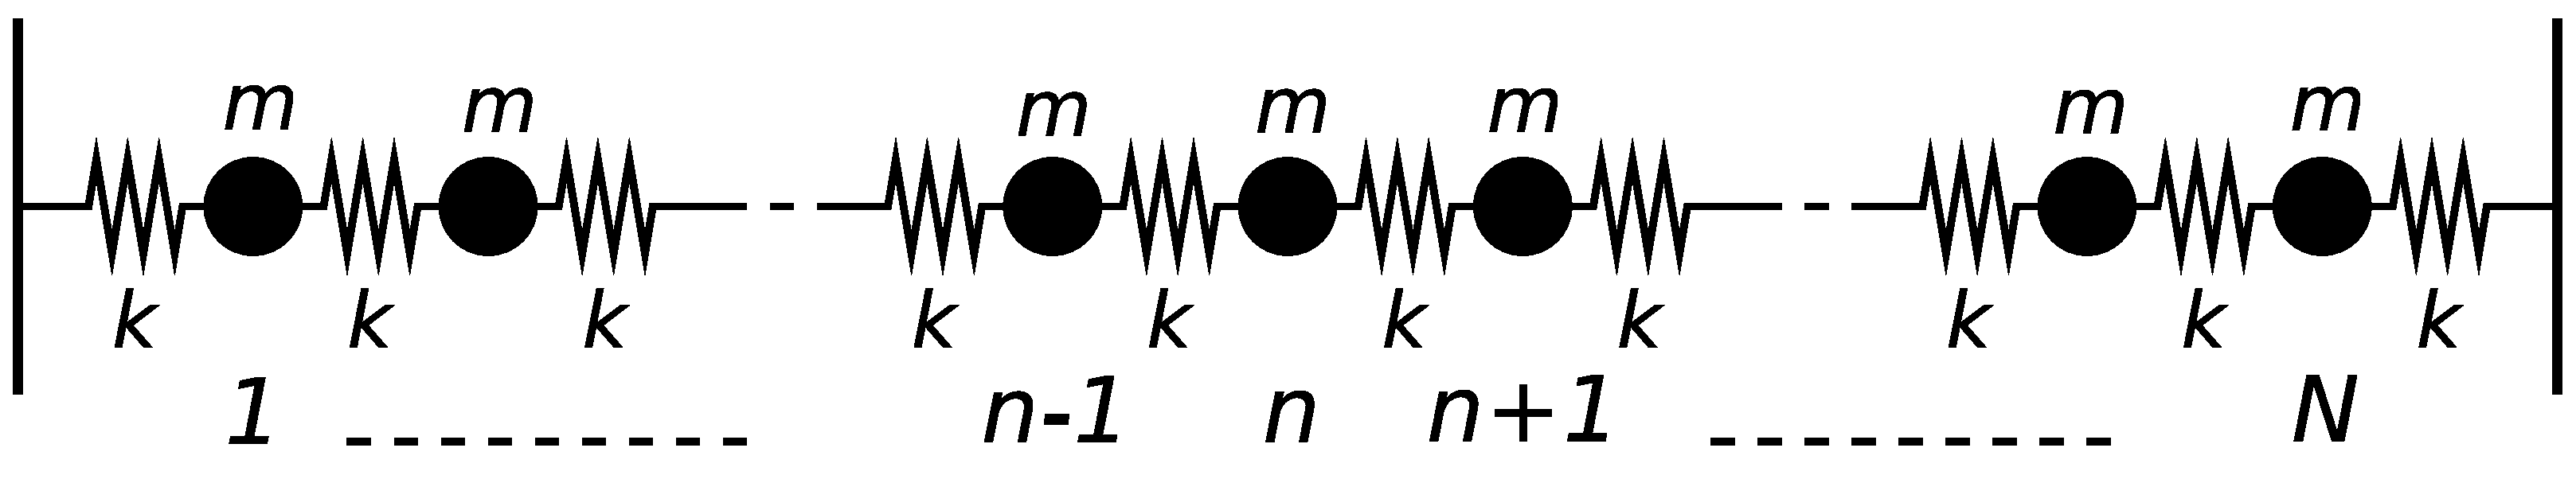
\includegraphics[width=\textwidth]{ej1-11}
\end{minipage}
\begin{enumerate}
	\item Escriba la ecuación de movimiento transversal para la partícula enésima usando la aproximación de ángulos pequeños.
	\item Proponga una solución de la forma:
	\[
		\Psi_{n}^{(p)}(t)=A^{(p)}\cos\left(nk^{(p)}a+\alpha^{(p)}\right)\cos\left(\omega^{(p)}t+\phi^{(p)}\right)
	\]
	Halle la relación de dispersión y grafíquela.
	¿Depende esta relación de las condiciones de contorno?
	¿Cuánto vale la frecuencia más baja?
	¿Qué representa dicho modo? 
	\item Obtenga las frecuencias correspondientes a los modos normales cuando ambos extremos están libres (atención: ¿cómo sería un ``extremo libre'' en esta configuración?) y escriba la solución general para la masa enésima. 
	\item Ídem. anterior, pero con el extremo izquierdo libre y el derecho fijo a la pared. 
	\item Particularice los resultados de los dos ítems anteriores para el caso en que $N=3$.
\end{enumerate}



\item
\begin{minipage}[t][2cm]{0.6\textwidth}
 Considere el sistema de péndulos acoplados de la figura. 
\end{minipage}
\begin{minipage}[c][2cm][t]{0.35\textwidth}
  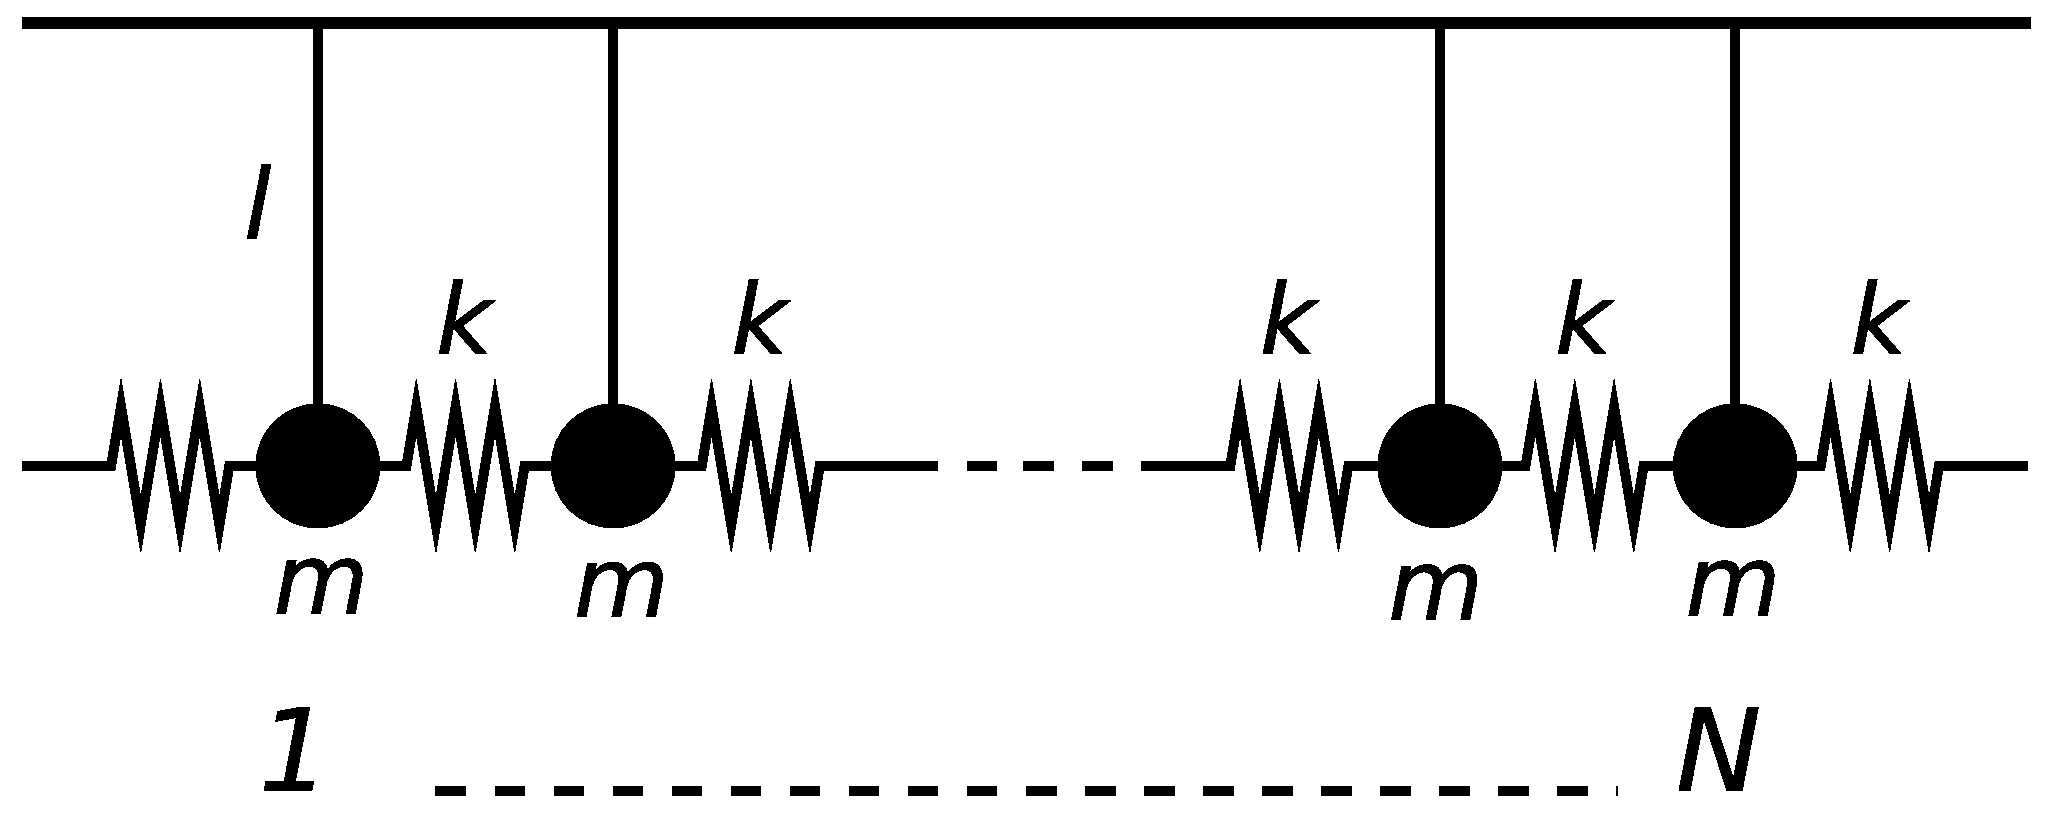
\includegraphics[width=\textwidth]{ej1-12}
\end{minipage}
\begin{enumerate}
	\item Escriba la ecuación de movimiento. Proponga una solución semejante a la del problema anterior y halle la relación de dispersión. Compárela con la obtenida en el problema anterior.
	¿Cuánto vale la frecuencia más baja?
	¿Qué representa dicho modo? 
	\item Obtenga las frecuencias correspondientes a los modos normales cuando los resortes de los extremos están fijos y dé las condiciones iniciales para excitar el primer armónico. 
	\item Ídem anterior, pero para el caso en que uno de los resortes de los extremos está libre. 
\end{enumerate}



\end{enumerate}

\end{document}
